
The basis functions for this element is presented in Section~\ref{ss:Q1Q1bb_3D}.
This element is presented in Karabelas \etal (2020) \cite{kahp20}. 

There are two bubble functions/nodes per element so we then have 
\begin{lstlisting}
NV=nnx*nny*nnz+2*nel 
NP=nnx*nny*nnz
\end{lstlisting}
For a 8x8x8=512 element grid, there are $9^3=729$ nodes, and 1024 bubble nodes.
We then have $3\cdot 729=2157$ $Q_1$ velocity dofs and 3072 velocity dofs attached 
to the bubbles.
Since the bubble nodes are stored last the structure of the matrix is as follows:
\begin{center}
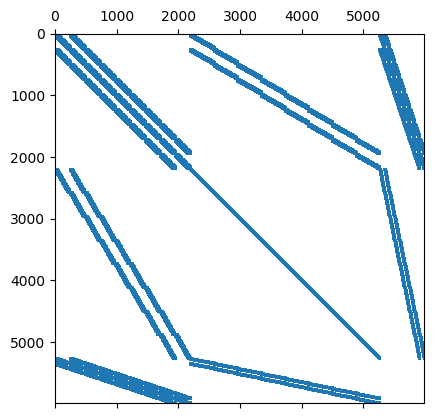
\includegraphics[width=6cm]{python_codes/fieldstone_82/results/matrix_8x8x8_bef_bc}
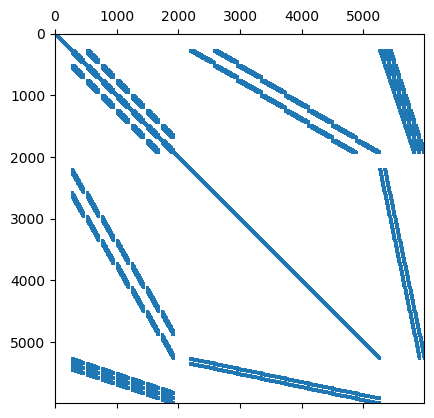
\includegraphics[width=6cm]{python_codes/fieldstone_82/results/matrix_8x8x8_aft_bc}\\
{\captionfont Sparsity pattern of the matrix for a 8x8x8 grid.
NV= 1753, NP=729.\\ Left:
before boundary conditions are applied. 
Right: after boundary conditions are applied.} 
\end{center}


%......................................
\subsubsection*{Manufactured solution (bench=1)}

This benchmark begins by postulating a polynomial solution 
to the 3D Stokes equation (see Dohrmann \& Bochev (2004) \cite{dobo04}):
\begin{equation}
\vec{\upnu}(x,y,z)
=
\left(
\begin{array}{c}
x+x^2+xy+x^3y \\
y + xy + y^2 + x^2 y^2\\
-2z - 3xz - 3yz - 5x^2 yz
\end{array}
\right)
\label{eqbur2}
\end{equation}
and
\begin{equation}
p(x,y,z) = xyz + x^3 y^3z - 5/32
\end{equation}
The corresponding right-hand side is computed in Section~\ref{mms3}.
The domain is a unit cube and velocity boundary conditions
simply use Eq. (\ref{eqbur2}).
Note that the pressure fulfills $\int_\Omega p(x,y,z) dV = 0.$

\begin{center}
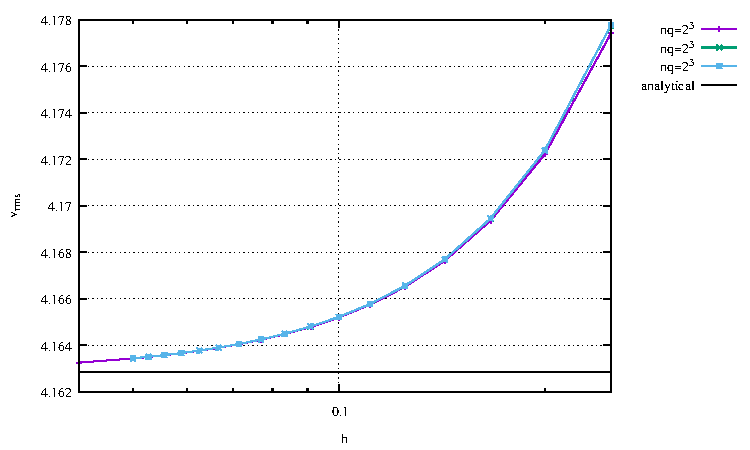
\includegraphics[width=8cm]{python_codes/fieldstone_82/results/bench1/vrms.pdf}
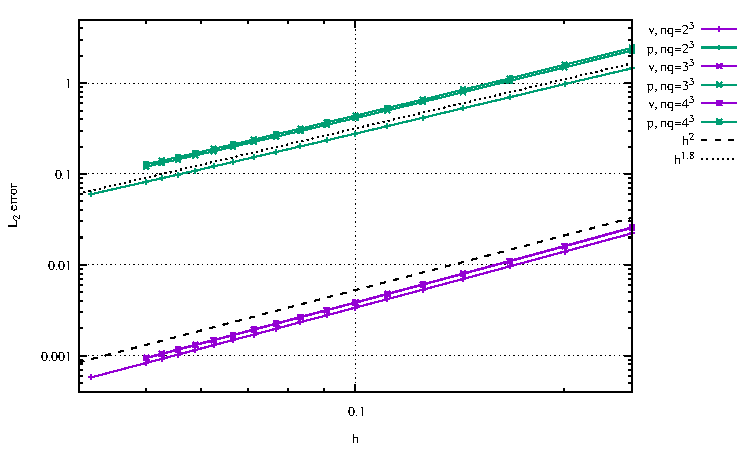
\includegraphics[width=8cm]{python_codes/fieldstone_82/results/bench1/conv.pdf}\\
{\captionfont Results obtained for three levels of quadrature, with $\beta=0$ (i.e.
viscosity is constant and equal to 1).}
\end{center}

Somewhat surprisingly, the pressure convergence is not exactly quadratic but seems to be
around 1.8. Also, the $2\times 2\times 2$ 
quadrature yields better results than the $3\times 3\times 3$ or $4\times 4 \times 4$.

%......................................
\subsubsection*{Horizontal shear (bench=2)}

This is a simple kinematical test: gravity is set to zero, no boundary 
conditions on the sides and $\vec\upnu=(-1,0,0)$ prescribed on the top, and 
$\vec\upnu=(+1,0,0)$ prescribed on the bottom.

\begin{center}
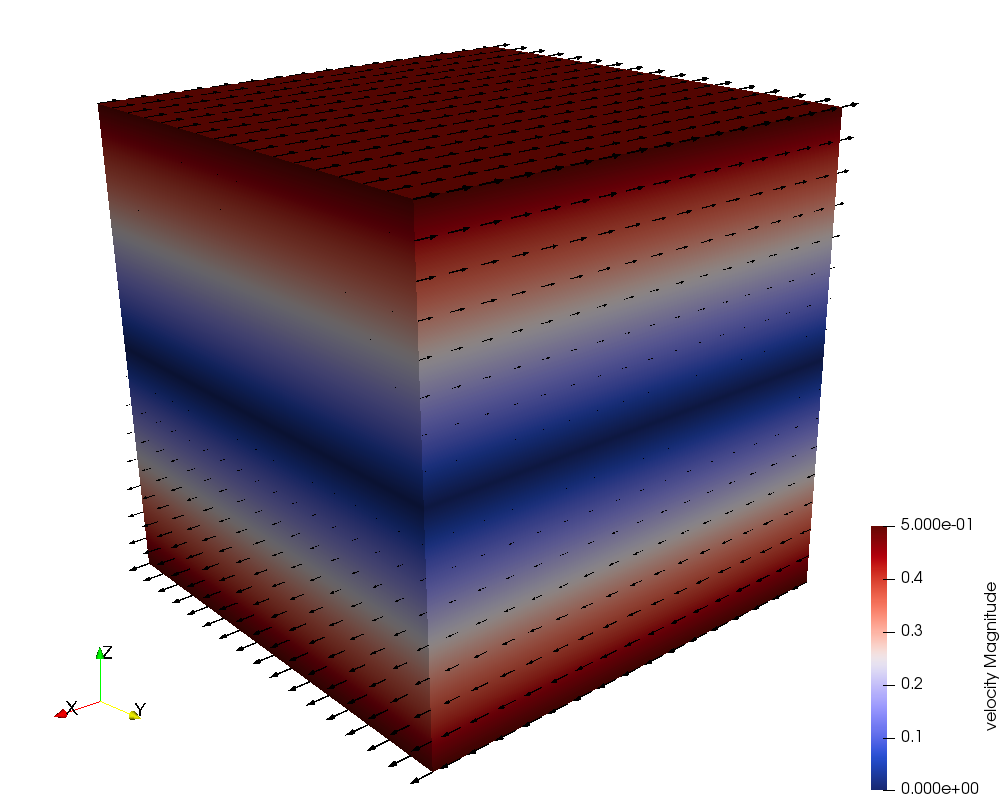
\includegraphics[width=6cm]{python_codes/fieldstone_82/results/bench2/vel}
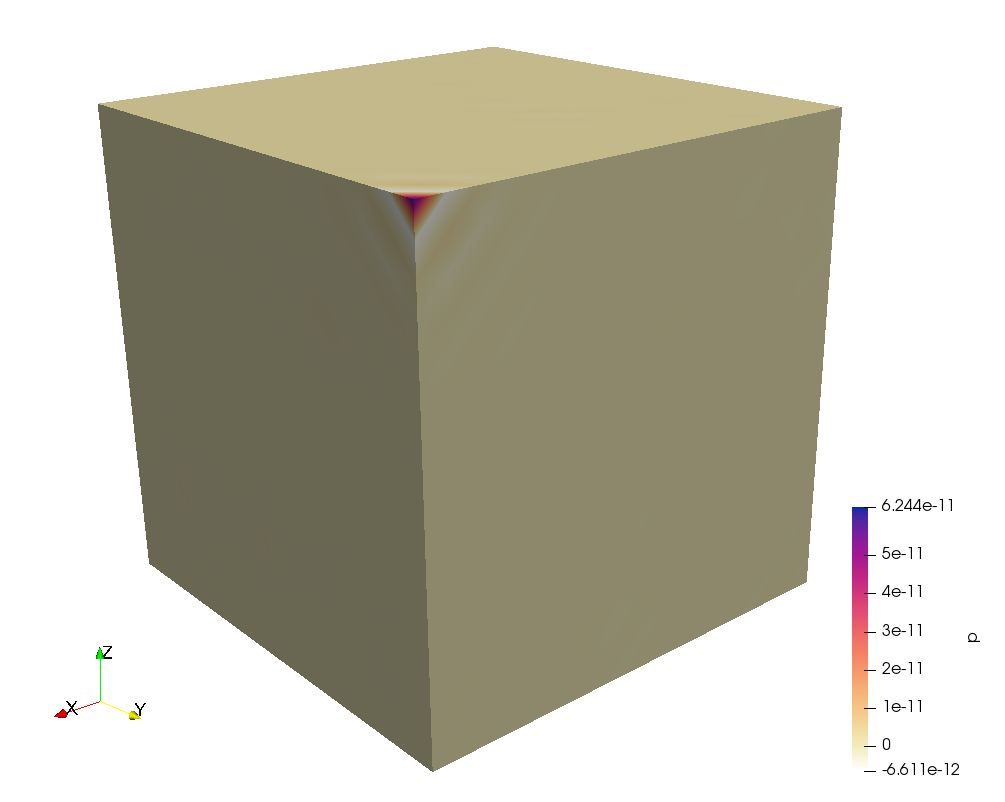
\includegraphics[width=6cm]{python_codes/fieldstone_82/results/bench2/press}\\
{\captionfont 20x20x20 mesh.} 
\end{center}

%......................................
\subsubsection*{Stokes sphere (bench=3)}

This is the benchmark of Section~\ref{ss:stokes_sphere3D}.
A sphere of radius 0.123456789 is placed in the middle of the domain. 
It has a density excess $\delta\rho=0.01$
with respect to the surrounding fluid which has a density $\rho_{fluid}=1$. 
The sphere viscosity is 1000 why the fluid viscosity is 1.
Boundary conditions are no slip on all sides. Gravity is $\vec{g}=-\vec{e}_z$.

\begin{center}
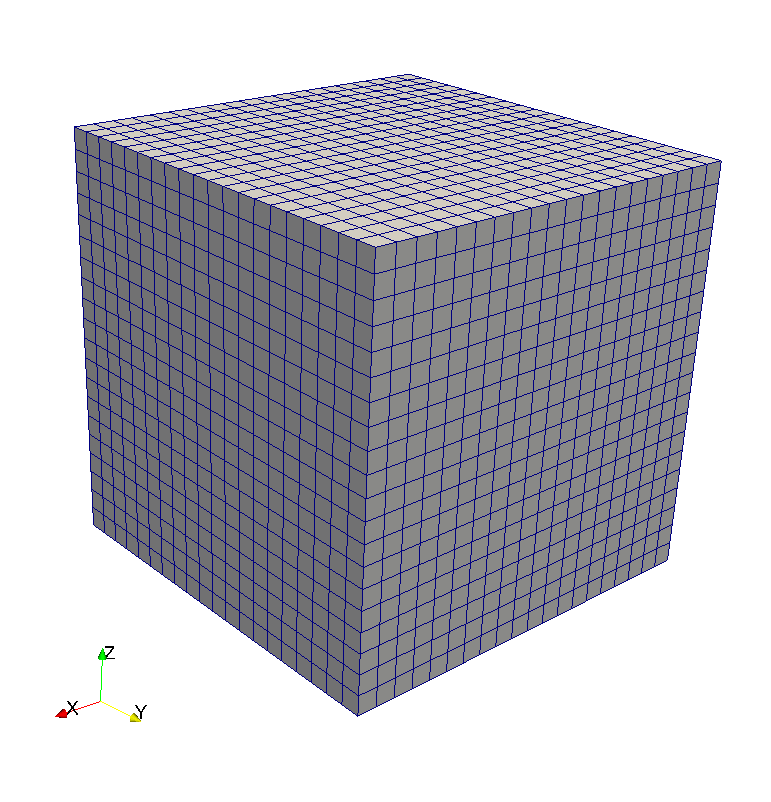
\includegraphics[width=5cm]{python_codes/fieldstone_82/results/bench3/grid.png}
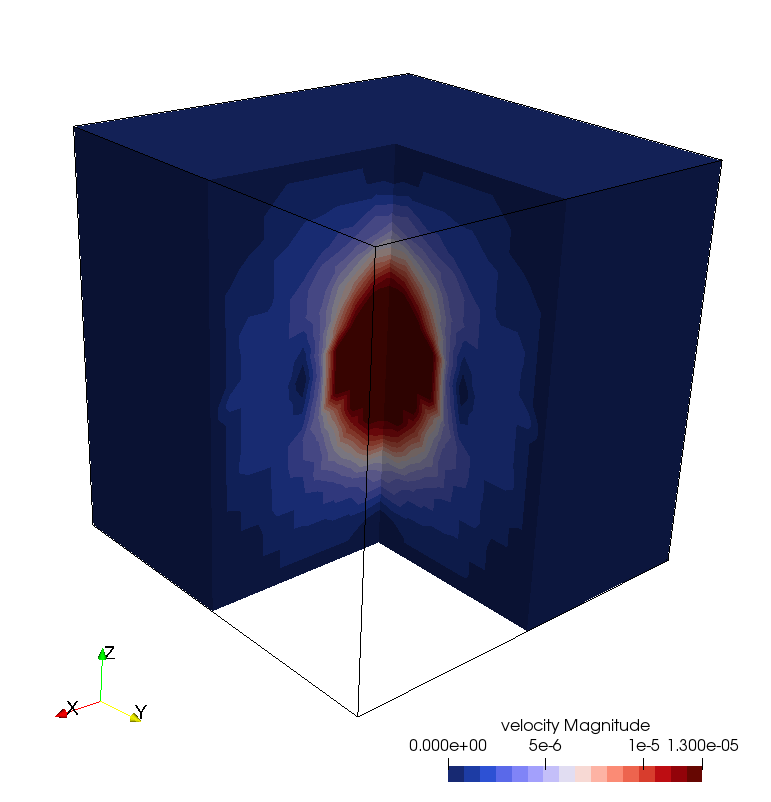
\includegraphics[width=5cm]{python_codes/fieldstone_82/results/bench3/vel.png}
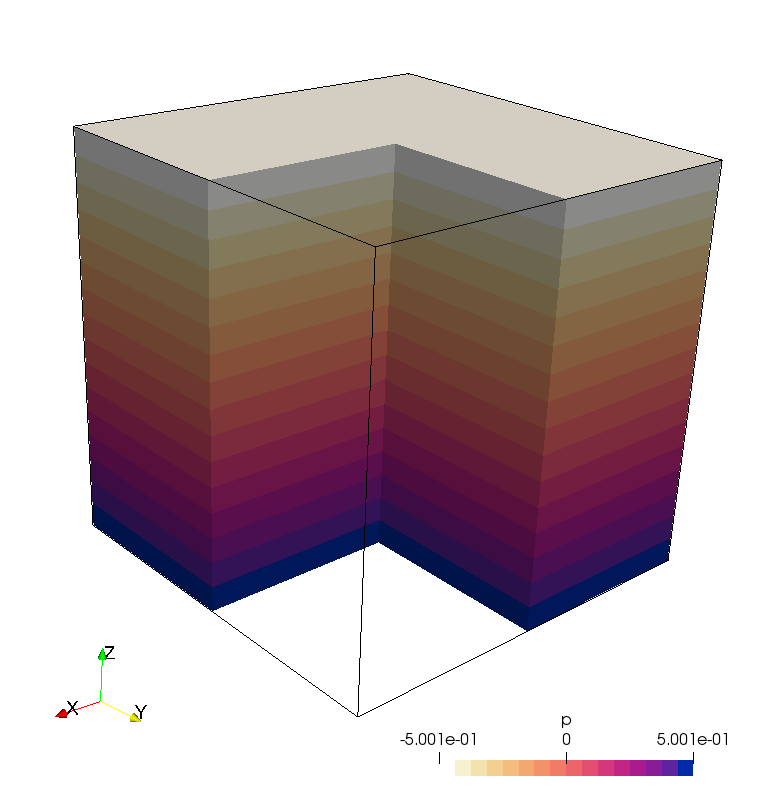
\includegraphics[width=5cm]{python_codes/fieldstone_82/results/bench3/press.png}\\
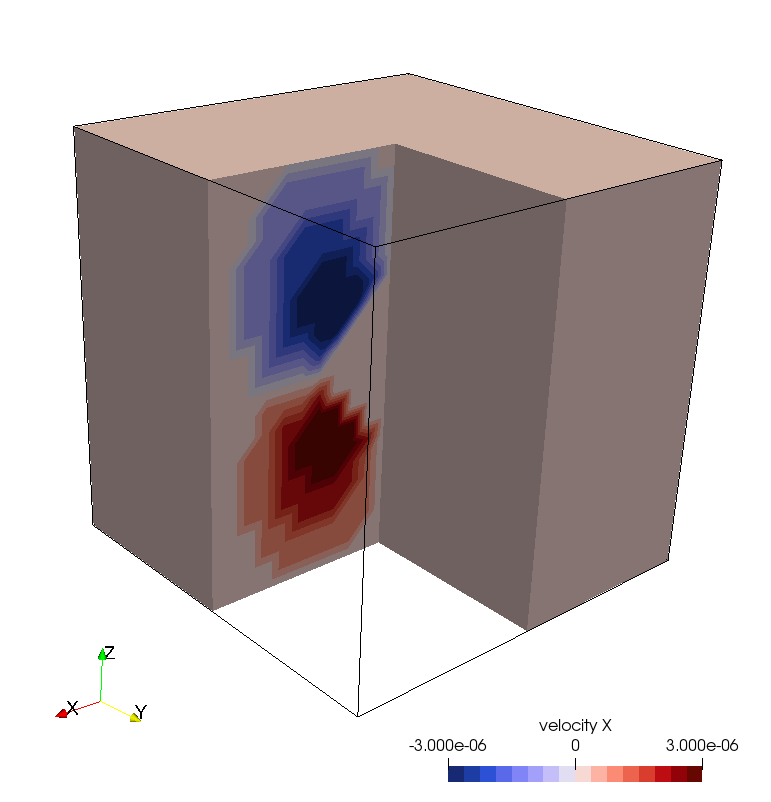
\includegraphics[width=5cm]{python_codes/fieldstone_82/results/bench3/u.png}
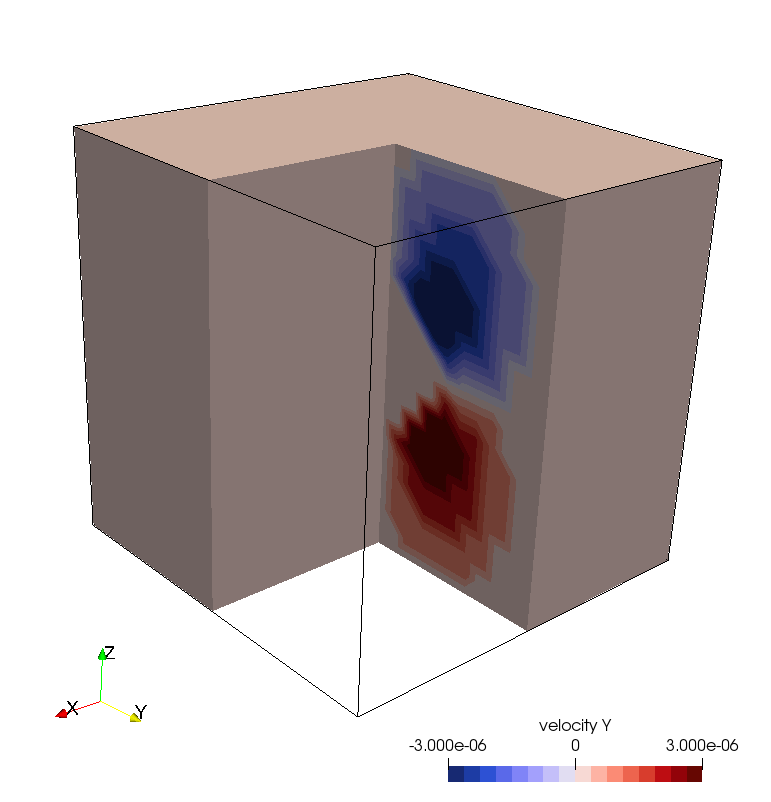
\includegraphics[width=5cm]{python_codes/fieldstone_82/results/bench3/v.png}
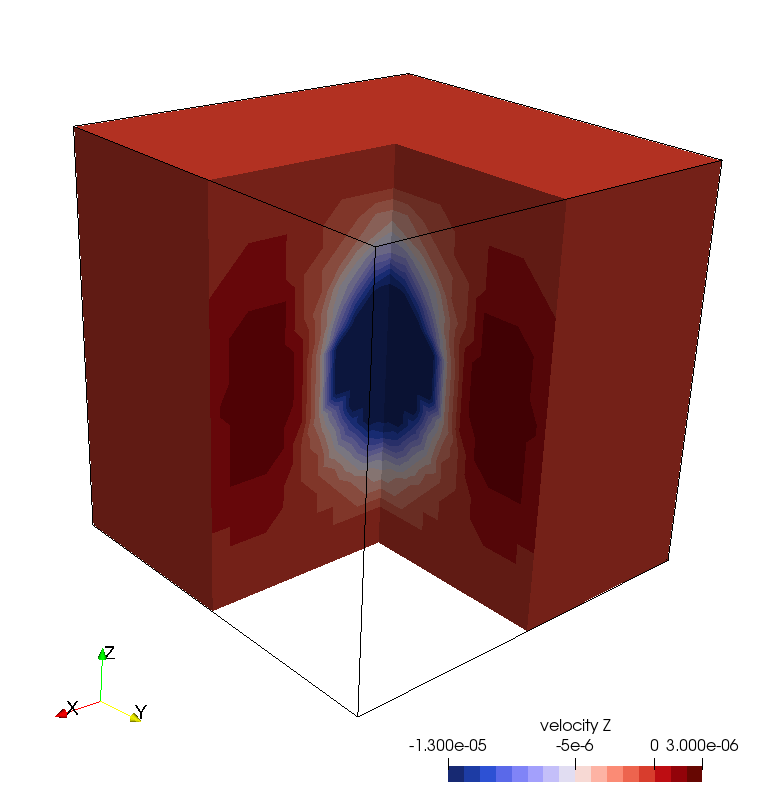
\includegraphics[width=5cm]{python_codes/fieldstone_82/results/bench3/w.png}\\
{\captionfont Resolution $20\times 20\times 20$. Quadrature $2\times 2 \times 2$.} 
\end{center}

All velocity and pressure statistics are presented in Section~\ref{ss:stokes_sphere3D}.

\begin{center}
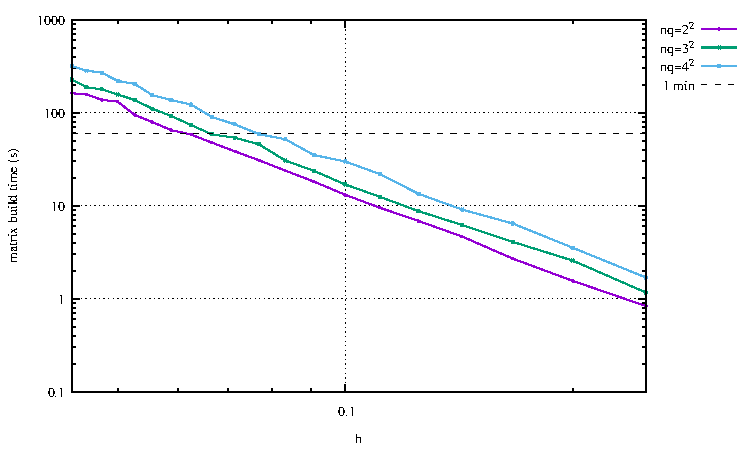
\includegraphics[width=8cm]{python_codes/fieldstone_82/results/bench3/build.pdf}
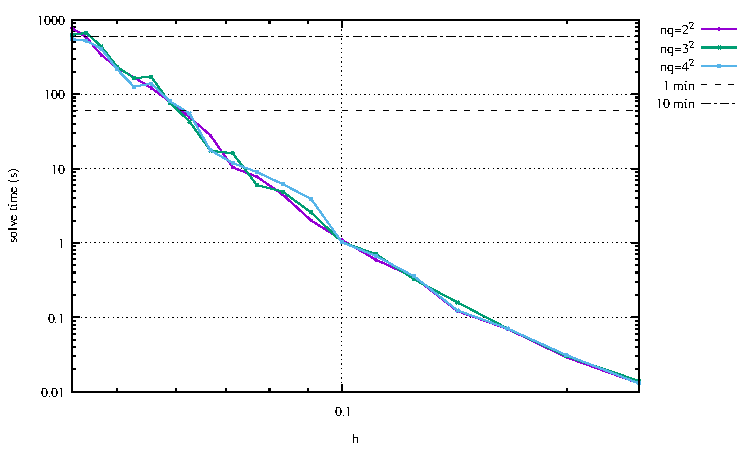
\includegraphics[width=8cm]{python_codes/fieldstone_82/results/bench3/solve.pdf}\\
{\captionfont Matrix build and solve time as a function of $h$.}
\end{center}

%......................................
\subsubsection*{Sinking cube (bench=4)}

This is the same experiment as the Stokes sphere with the exception of the geometry of the sinker which 
is 0.25x0.25x0.25 in size so that its edges align with boundary edges for 8x8x8, 16x16x16 and 24x24x24 meshes.
Reduced density is used in order to remove the lithostatic pressure signal.
 
\begin{center}
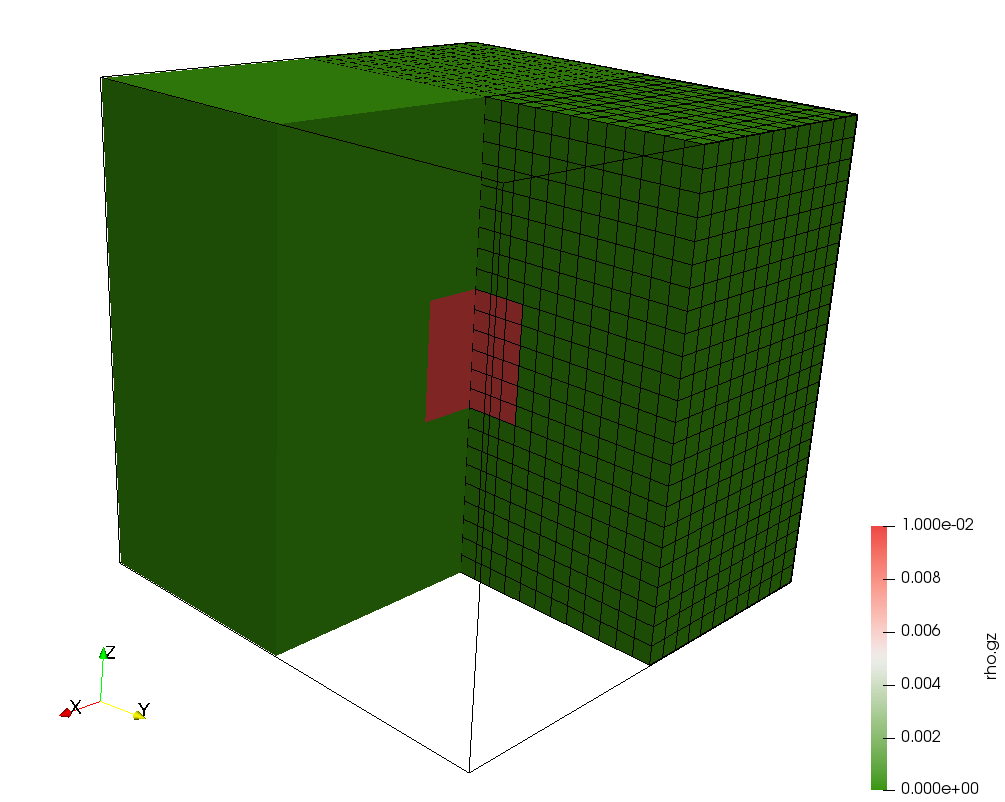
\includegraphics[width=8cm]{python_codes/fieldstone_82/results/bench4/rho}
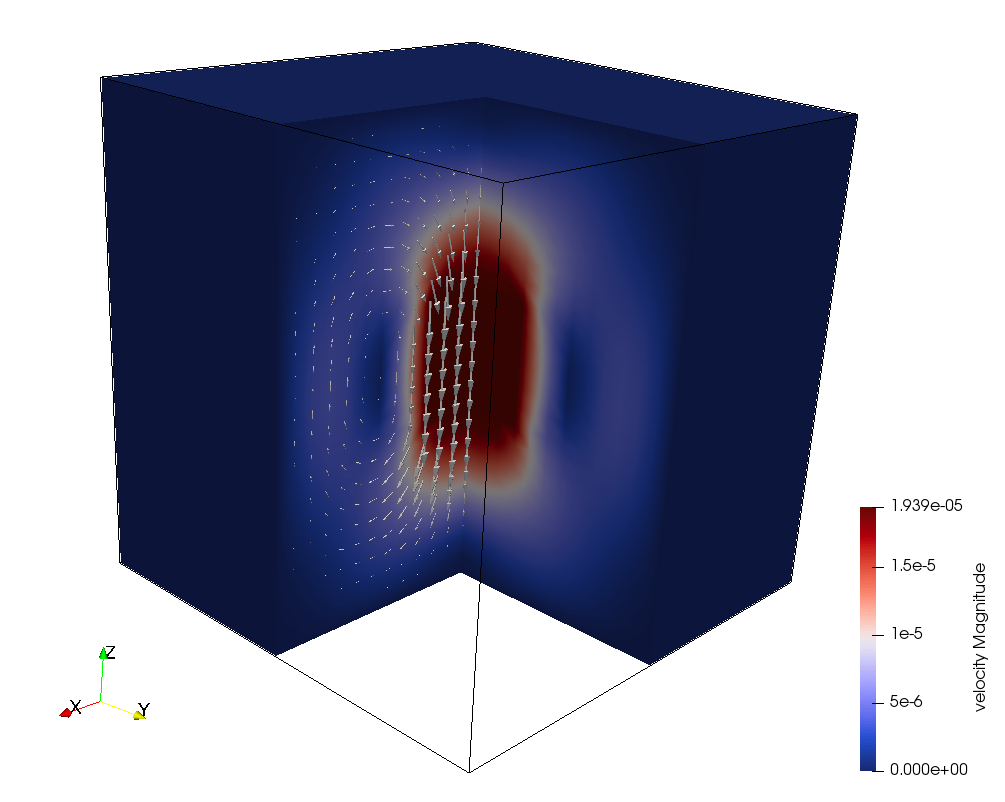
\includegraphics[width=8cm]{python_codes/fieldstone_82/results/bench4/vel}\\
{\captionfont resolution 24x24x24 elements.}
\end{center}

The velocity and pressures are interpolated on 100 points on the four diagonals of the cube
as a way to verify the symmetry of the solution (the bubbles rely on the basis 
functions of nodes 0 and 6 afterall!). $2^3$ quadrature points per element are used. 

\begin{center}
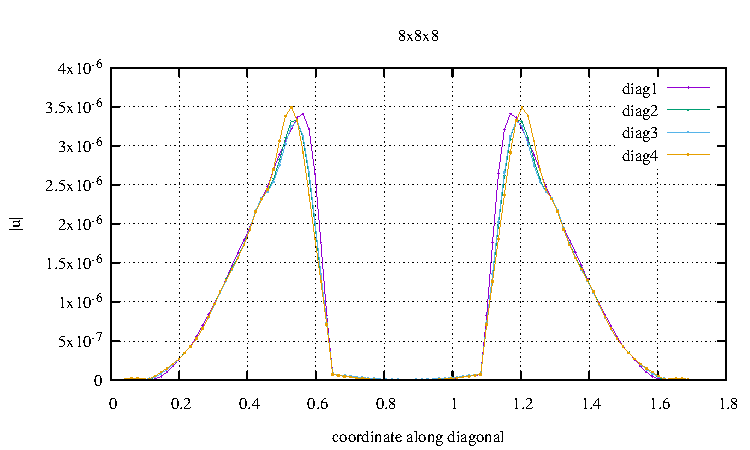
\includegraphics[width=5.5cm]{python_codes/fieldstone_82/results/bench4/u_08}
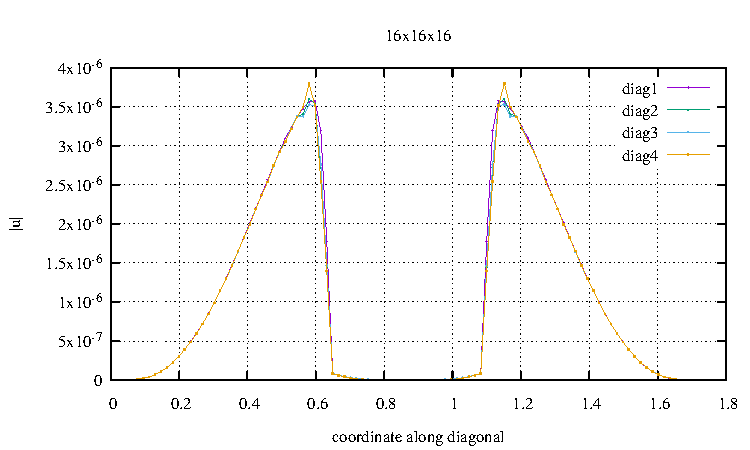
\includegraphics[width=5.5cm]{python_codes/fieldstone_82/results/bench4/u_16}
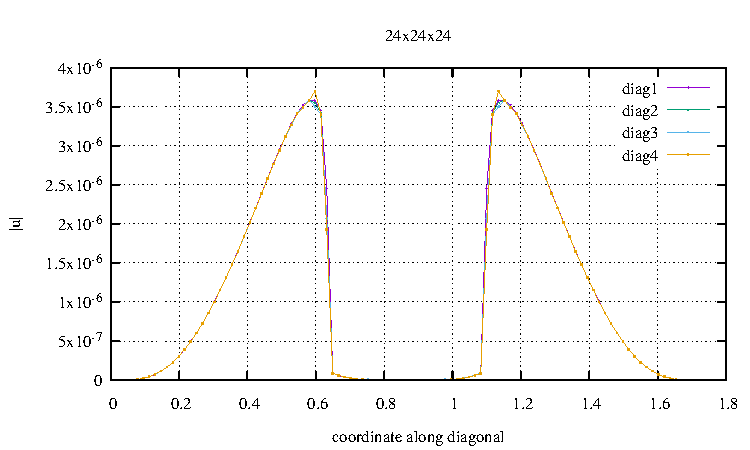
\includegraphics[width=5.5cm]{python_codes/fieldstone_82/results/bench4/u_24}\\
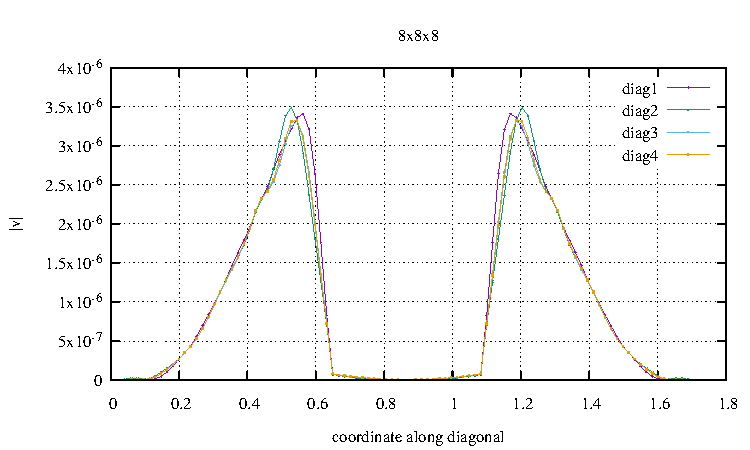
\includegraphics[width=5.5cm]{python_codes/fieldstone_82/results/bench4/v_08}
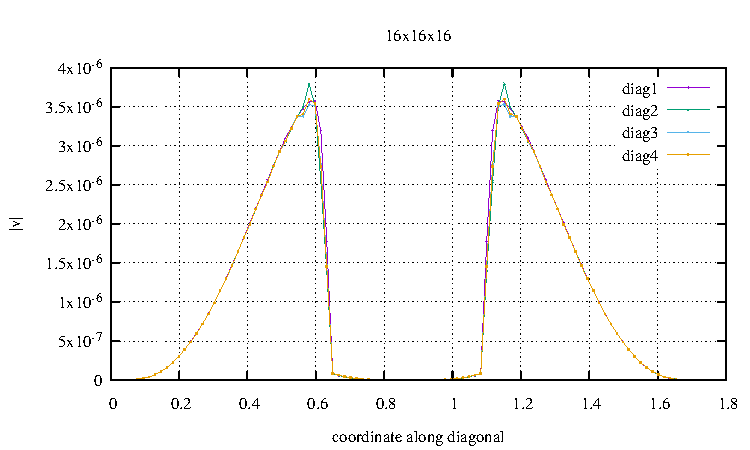
\includegraphics[width=5.5cm]{python_codes/fieldstone_82/results/bench4/v_16}
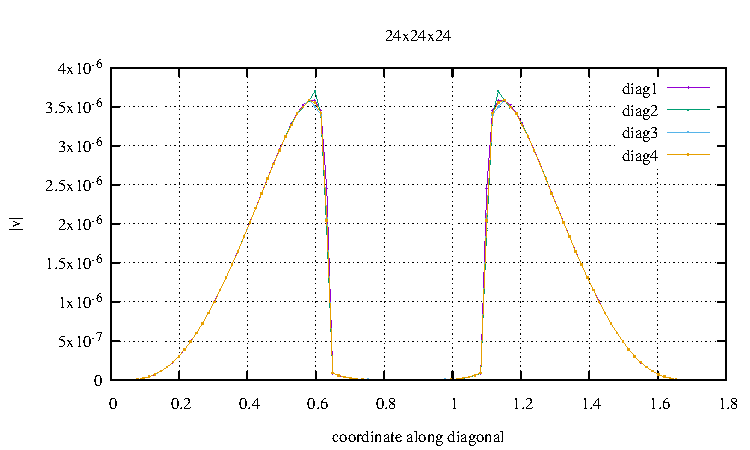
\includegraphics[width=5.5cm]{python_codes/fieldstone_82/results/bench4/v_24}\\
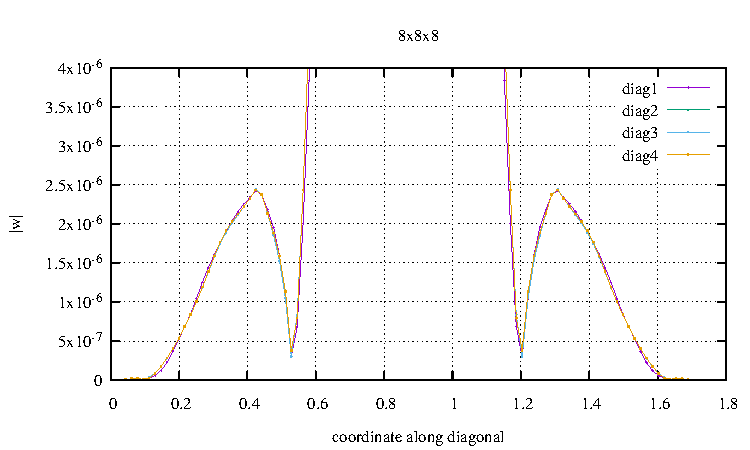
\includegraphics[width=5.5cm]{python_codes/fieldstone_82/results/bench4/w_08}
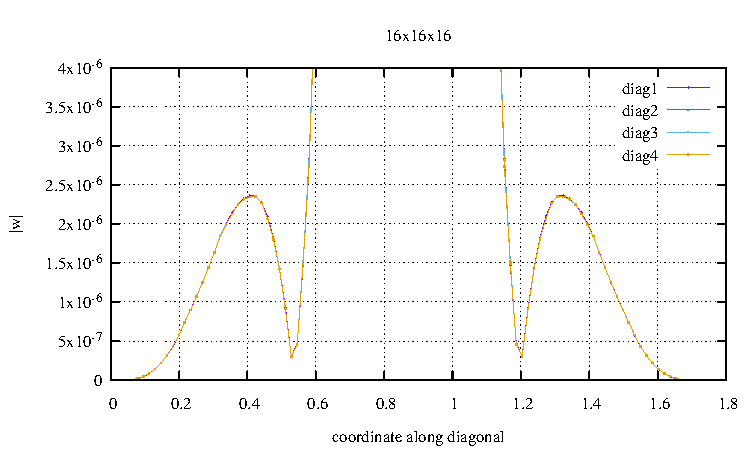
\includegraphics[width=5.5cm]{python_codes/fieldstone_82/results/bench4/w_16}
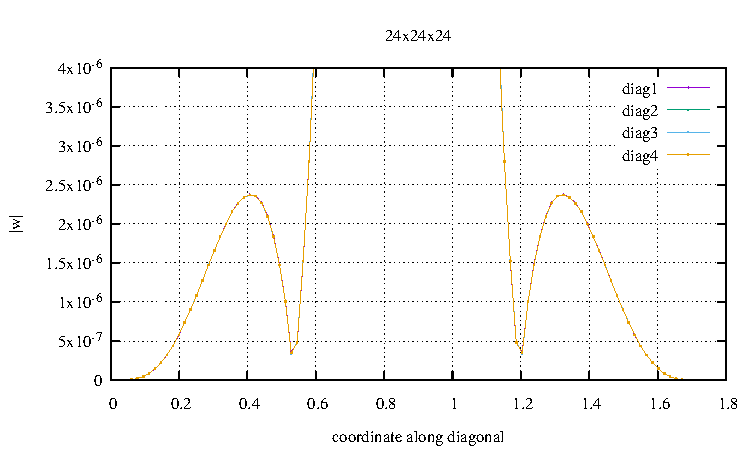
\includegraphics[width=5.5cm]{python_codes/fieldstone_82/results/bench4/w_24}\\
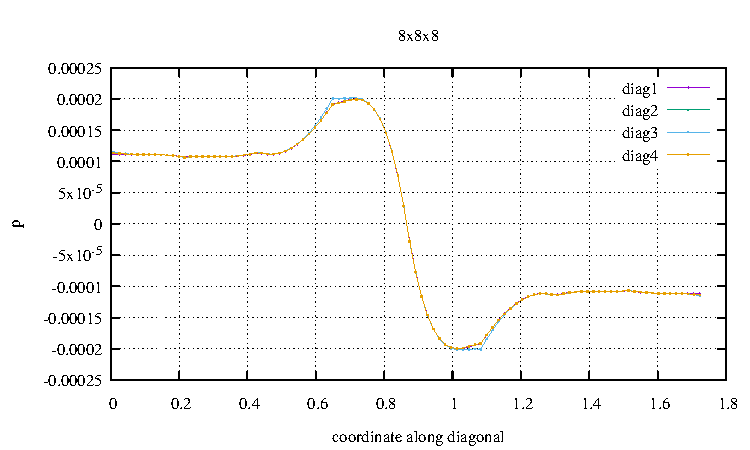
\includegraphics[width=5.5cm]{python_codes/fieldstone_82/results/bench4/p_08}
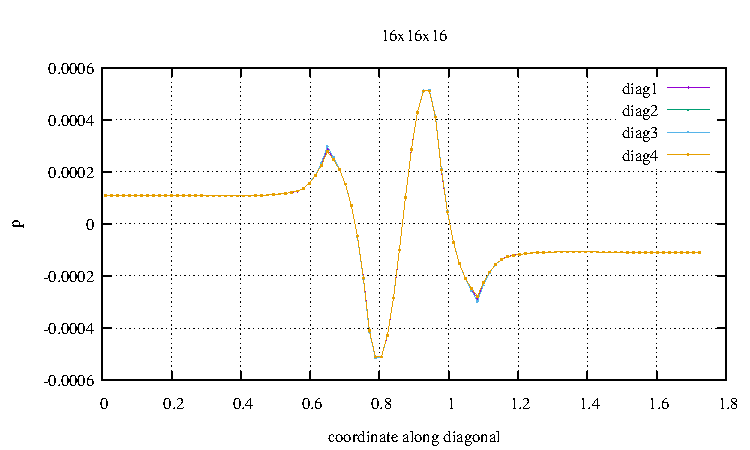
\includegraphics[width=5.5cm]{python_codes/fieldstone_82/results/bench4/p_16}
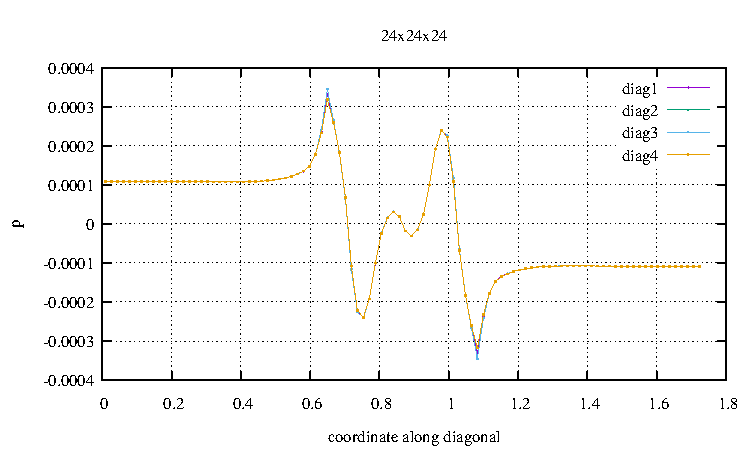
\includegraphics[width=5.5cm]{python_codes/fieldstone_82/results/bench4/p_24}\\
{\captionfont Left to right: increasing resolution}
\end{center}

We can also plot the velocity and pressure fields on a vertical line passing 
through the middle of the block:
\begin{center}
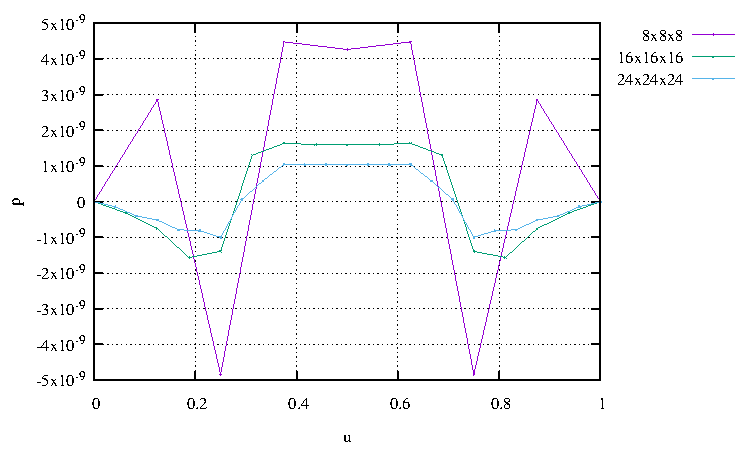
\includegraphics[width=5.5cm]{python_codes/fieldstone_82/results/bench4/vert_u}
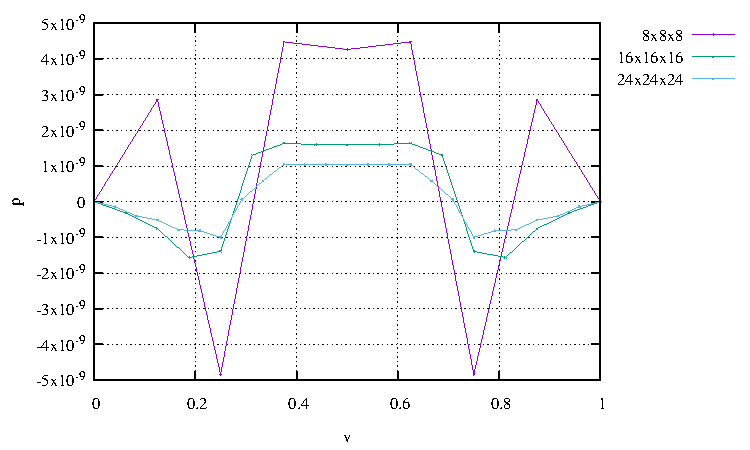
\includegraphics[width=5.5cm]{python_codes/fieldstone_82/results/bench4/vert_v}
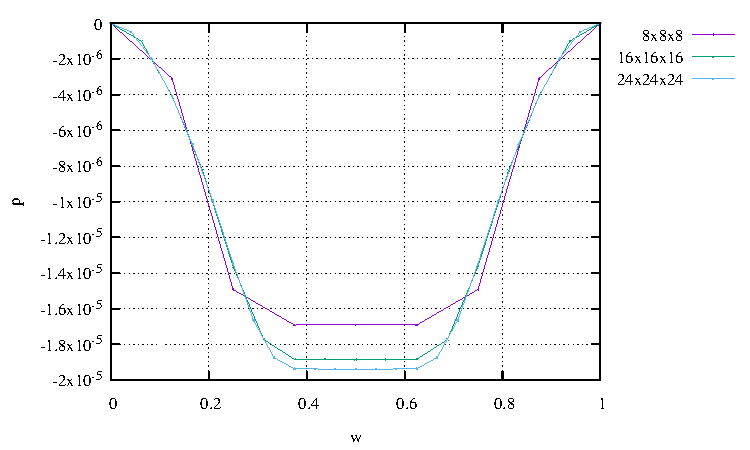
\includegraphics[width=5.5cm]{python_codes/fieldstone_82/results/bench4/vert_w}
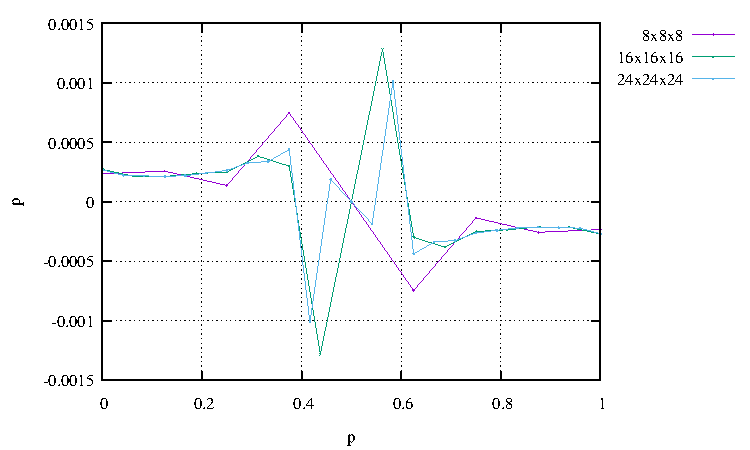
\includegraphics[width=5.5cm]{python_codes/fieldstone_82/results/bench4/vert_p}
\end{center}
We see that unfortunately the resolution 24x24x24 is most certainly not high 
enough to speak of capturing the true solution of the problem...




%......................................
\subsubsection*{Manufactured solution (bench=5)}

We here consider the manufactured solution which is introduced in Section~\ref{ss:mms3Dgen}.
The velocity and pressure fields are:
\begin{eqnarray}
u(x,y,z) &=& x(1-x)(1-2y)(1-2z)\\
v(x,y,z) &=& (1-2x) y(1-y) (1-2z) \\
w(x,y,z) &=& -2(1-2x)(1-2y)z(1-z) \\
p(x,y,z) &=& (2x-1)(2y-1)(2z-1)
\end{eqnarray}
This flow field has the built-in property that there is no flux through the 
boundaries.

\begin{center}
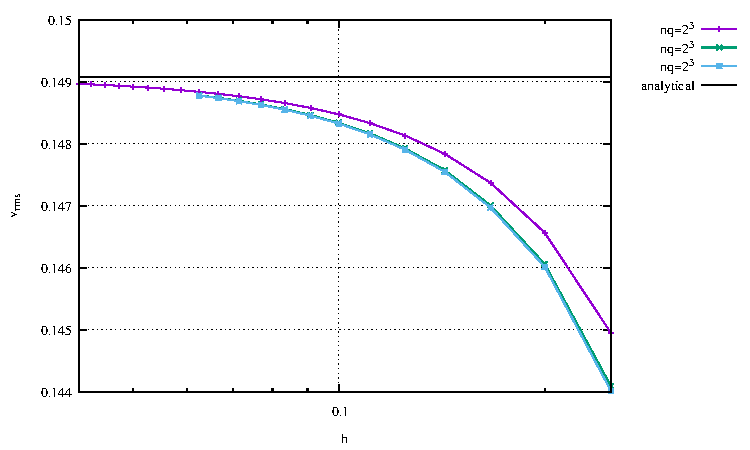
\includegraphics[width=8cm]{python_codes/fieldstone_82/results/bench5/vrms.pdf}
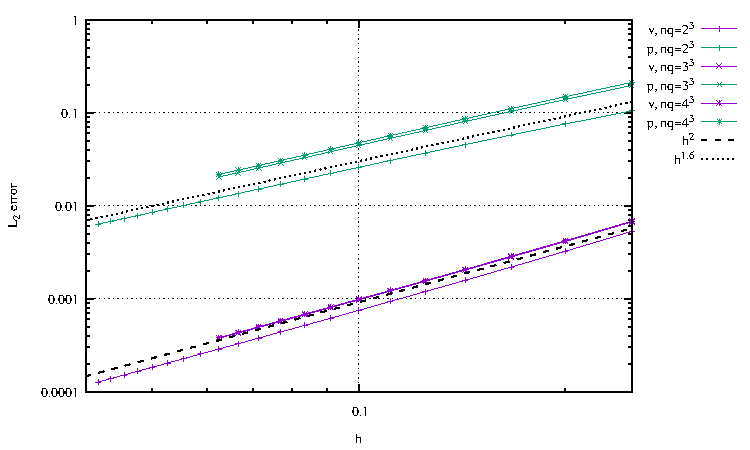
\includegraphics[width=8cm]{python_codes/fieldstone_82/results/bench5/conv.pdf}\\
{\captionfont Results obtained for three levels of quadrature.}
\end{center}


\begin{center}
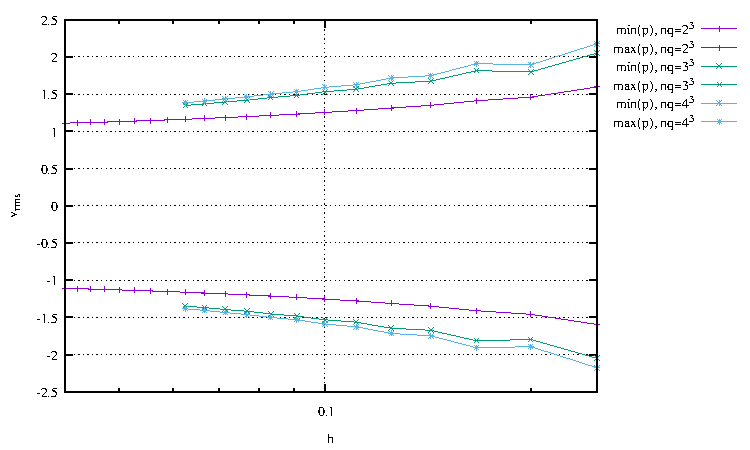
\includegraphics[width=8cm]{python_codes/fieldstone_82/results/bench5/p_stats.pdf}
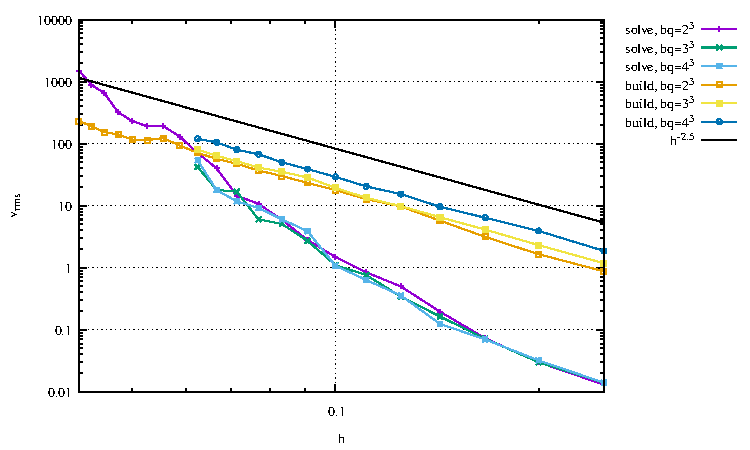
\includegraphics[width=8cm]{python_codes/fieldstone_82/results/bench5/times.pdf}
\end{center}







